\documentclass[twoside,twocolumn]{article}

\usepackage{blindtext} % Package to generate dummy text throughout this template 
\usepackage{graphicx}
\usepackage[sc]{mathpazo} % Use the Palatino font
\usepackage[T1]{fontenc} % Use 8-bit encoding that has 256 glyphs
\linespread{1.05} % Line spacing - Palatino needs more space between lines
\usepackage{microtype} % Slightly tweak font spacing for aesthetics

\usepackage[english]{babel} % Language hyphenation and typographical rules

\usepackage[hmarginratio=1:1,top=32mm,columnsep=20pt]{geometry} % Document margins
\usepackage[hang, small,labelfont=bf,up,textfont=it,up]{caption} % Custom captions under/above floats in tables or figures
\usepackage{booktabs} % Horizontal rules in tables
\usepackage{graphicx}
\usepackage{lettrine} % The lettrine is the first enlarged letter at the beginning of the text

\usepackage{enumitem} % Customized lists
\setlist[itemize]{noitemsep} % Make itemize lists more compact

\usepackage{abstract} % Allows abstract customization
\renewcommand{\abstractnamefont}{\normalfont\bfseries} % Set the "Abstract" text to bold
\renewcommand{\abstracttextfont}{\normalfont\small\itshape} % Set the abstract itself to small italic text

\usepackage{titlesec} % Allows customization of titles

\titleformat{\section}[block]{\large\scshape\centering}{\thesection.}{1em}{} % Change the look of the section titles
\titleformat{\subsection}[block]{\large}{\thesubsection.}{1em}{} % Change the look of the section titles

\usepackage{fancyhdr} % Headers and footers
\pagestyle{fancy} % All pages have headers and footers
\fancyhead{} % Blank out the default header
\fancyfoot{} % Blank out the default footer
\fancyhead[C]{Datos no estructurados $\bullet$ Noviembre 2021 $\bullet$ } % Custom header text
\fancyfoot[RO,LE]{\thepage} % Custom footer text

\usepackage{titling} % Customizing the title section

\usepackage{hyperref} % For hyperlinks in the PDF

%----------------------------------------------------------------------------------------
%	TITLE SECTION
%----------------------------------------------------------------------------------------
\providecommand{\keywords}[1]{
  \small	
  \textbf{\textit{\quad \quad Keywords: }} #1}

\providecommand{\pclave}[1]{
  \small	
  \textbf{\textit{\quad \quad Palabras Clave: }} #1}

%Idiomas: \selectlanguage{english} \selectlanguage{spanish}

\begin{document}

\title{Trabajo Encargado N°1: Datos no estructurados}

\begin{titlepage}
\begin{figure}[htb]
\begin{center}

\includegraphics[width=5cm]{imagenes/logo.png}
\end{center}
\end{figure}
\vspace*{-0.25in}
\begin{center}
\large{UNIVERSIDAD PRIVADA DE TACNA}\\
\vspace*{-0.025in}
INGENIERIA DE SISTEMAS  \\

\vspace*{0.5in}
\begin{large}
TITULO:\\
\end{large}

\vspace*{0.1in}
\begin{Large}
\textbf{Datos no estructurados} \\
\end{Large}

\vspace*{0.3in}
\begin{Large}
\textbf{CURSO:} \\
\end{Large}

\vspace*{0.1in}
\begin{large}
Base de Datos II\\
\end{large}

\vspace*{0.3in}
\begin{Large}
\textbf{DOCENTE:} \\
\end{Large}

\vspace*{0.1in}
\begin{large}
 Ing. Patrick Cuadros Quiroga\\
\end{large}

\vspace*{0.2in}
\vspace*{0.1in}
\begin{large}

Integrantes: \\
\begin{flushleft}
Maldonado Cancapi, Carlos Alejandro\hfill(2018000660) \\
Huillca Aroni, Alfredo\hfill(2018060903)\\
Huallpa Huayachani, Alexander Junior\hfill(2018062497)\\
Anahua Huayhua, Jenny Karen\hfill(2018062150)\\
Condori Ramirez, Laura Soledad\hfill(2006028408)\\
Soto Rodriguez, Daniela Duanet\hfill(2015051384)\\

\end{flushleft}
\end{large}

\vspace*{0.1in}
\begin{large}
Tacna - Perú\\
2021
\end{large}
\end{center}
\end{titlepage}

\setlength{\droptitle}{-4\baselineskip} % Move the title up

\pretitle{\begin{center}\Huge\bfseries} % Article title formatting
\posttitle{\end{center}} % Article title closing formatting
\title{Datos no estructurados} % Article title

\date{\today} % Leave empty to omit a date                     
\renewcommand{\maketitlehookd}{%

}

%----------------------------------------------------------------------------------------



% Print the title
\maketitle

%----------------------------------------------------------------------------------------
%	ARTICLE CONTENTS
%----------------------------------------------------------------------------------------

\section{Resumen}

\lettrine[nindent=0em,lines=3]Los datos no estructurados podríamos
 decir que son datos binarios que no tienen una estructura comprensible
  para el lenguaje humano. Es una desorganización masiva de varios objetos
   que no tienen valor hasta que se identifican y almacenan de manera organizada. 
   Una vez que se ordenan, los elementos que conforman su contenido pueden ser 
   categorizados para obtener información. 
Este data supone alrededor de un 80\% de todo el
 existente en cualquier organización y su manejo resulta más complicado que el de los datos estructurados. Asimismo, no se puede almacenar en una herramienta de data tradicional, ya que sería imposible ajustarlos a las filas y columnas estandarizadas. 

Las empresas que consiguen extraer la información de estos datos
 cuentan con una gran ventaja competitiva. Y es que, esta tipología de datos aporta una visión mucho más completa y profunda del mercado: gracias a técnicas de data mining, que implican métodos de machine learning, inteligencia artificial y estadística, las empresas pueden conocer mejor, a través de la información no estructurada, los hábitos y los ritmos de compra, los patrones de comportamiento o las afinidades con determinados productos, entre otros. De hecho, la capacidad de extraer valor de ellos es uno de los principales motivos por los 
que el análisis del big data está evolucionando a gran velocidad. 


%------------------------------------------------

\section{Abstract}


Unstructured data is binary data 
that does not have a structure that
 can be understood by human language.
  It is a massive disorganization of 
  various objects that have no value 
  until they are identified and stored in an organized manner.
   Once sorted, the elements that make up your content can be categorized for information. 

This data represents around 80\% of all that exists in any organization
 and its management is more complicated than that of structured data.
  Also, it cannot be stored in a traditional data tool, as it would be impossible 
  to fit into standardized rows and columns. 

The companies that manage to extract the information from this data 
have a great competitive advantage. And it is that, this typology of 
data provides a much more complete and in-depth vision of the market: 
thanks to data mining techniques, which involve machine learning, artificial 
intelligence and statistics, companies can know better, through information 
not structure, buying habits and rhythms, behavior patterns or affinities with
 certain products, among others. In fact, the ability to extract value from them is one
 of the main reasons why big data analytics is evolving at such speed. 




%------------------------------------------------
\section{Introduccion}

Con el paso de los años, el análisis de datos ha ido ganando cada vez 
más relevancia para las organizaciones. Según afirman expertos en el área,
 para este año se estima que solo una parte de las empresas recolectará y analizará datos.
  A partir de ellos se podrá generar información sumamente valiosa.  

Esta data ocasionará que dichas empresas produzcan 430.000 millones de 
dólares por encima de aquellas que no se apoyen en la analítica. 
 Esto se debe a que el análisis de datos permite anticipar el futuro y 
 crear estrategias de gestión y de mercado con datos recopilados en tiempo real. 

Los datos no estructurados forman la mayor parte de la información 
relevante para una empresa u organización. Por lo general, son datos
 binarios que no tienen una estructura internar identificable. 
 Es decir, sí poseen una estructura interna, pero esta no está sujeta a 
 esquemas o modelos de datos predefinidos, por lo que estamos ante un conjunto
  desorganizado de varios objetos sin valor hasta que se identifican y se almacenan 
  de manera organizada. 

Sin embargo, no se pueden almacenar en una base de datos tradicional, 
sino que requieren bases de datos no relacionales o NoSQL. Pero una vez
 organizados en archivos, estos se pueden categorizar para poder obtener 
 información de ellos. 

\section{Desarrollo}

\subsection{EXTRACCION DE DATOS }

La toma de decisiones basada en datos puede ayudar a las empresas a mejorar 
su productividad en casi 6\%.
 Sin embargo, apenas 0.5\% de los datos del mundo se analiza y utiliza. Como 
 resultado, las empresas de todo el mundo están perdiendo prospectos masivos solo
  porque no pueden acceder a los datos requeridos en el momento adecuado. En esta 
  época, es crucial saber qué es la extracción de datos y ahí es donde la extracción 
  de bases de datos puede ser útil y volverse importante. Le ayuda a recuperar datos 
  y aprovecharlos al máximo para tomar decisiones comerciales bien informadas. 
  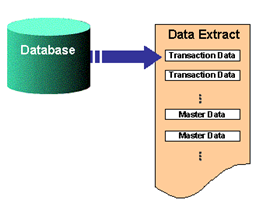
\includegraphics[width=7cm, height=7cm]{imagenes/1.png}


   
\subsection{¿Qué es la extracción de bases de datos?}

La extracción de bases de datos es un proceso de recuperación de datos de bases de datos dispares. En la mayoría de los casos, las empresas extraer datos para procesarlo más o transferirlo a otro repositorio para almacenamiento, como un almacén de datos o un lago de datos.
Por ejemplo, puede realizar algunos cálculos en los datos (como agregar información de ventas) y almacenar el resultado en su almacén de datos. Este procedimiento se llama ETL (Extraer, transformar y cargar). Y, la extracción es la primera etapa importante en ETL.
Beneficios de la extracción de bases de datos
La extracción de la base de datos ayuda a reconocer qué información es más valiosa para lograr sus objetivos comerciales, impulsando el proceso general de ETL. Puede extraer información útil oculta en desestructurado, semi-estructurado o fuentes de datos estructurados, como información del cliente.
Desafíos de extracción de bases de datos
Los siguientes son los desafíos clave de la extracción de bases de datos:

\begin{itemize}
    \item 	Datos no estructurados / semiestructurados 
    \item 	Problemas de compatibilidad
    \item 	Los datos sin procesar de varias fuentes a menudo tienen problemas de calidad de datos como valores duplicados, redundancia o datos contradictorios y problemas de seguridad, los datos pueden incluir información confidencial como información personal de clientes o cualquier otra información privada. 
\end{itemize}


\subsection{Técnicas de extracción de bases de datos}
La mejor técnica de extracción de base de datos que seleccione
 depende del sistema de origen, además de sus requisitos comerciales
  en el entorno del repositorio de destino. Los dos métodos de extracción
   de bases de datos más utilizados son:


\subsubsection{Extracción completa}

Los datos se extraen completamente de la fuente en su estado
 actual cargando la tabla de origen en la ubicación de destino
  tal como está. La extracción completa implica la transferencia
   de datos en gran volumen, y eso aumenta la carga en el sistema fuente.
    

\subsubsection{Extracción incremental}
Solo se extraen los datos que se han actualizado o 
cambiado desde un evento pasado discreto. Este evento 
pasado podría ser la última extracción exitosa o datos 
actualizados. Sin embargo, esta técnica tiene un gran desafío.
 Necesita al menos alguna información para reconocer todos los 
 datos modificados desde este evento pasado específico para reconocer
  el cambio delta. Los datos de origen en sí pueden proporcionar esta 
  información (como una columna de aplicación que revela la última marca 
  de tiempo modificada), o podría haber un cambio en la tabla que ofrece 
  esta información mediante el uso de un mecanismo complementario apropiado
   para rastrear las variaciones además de las transacciones iniciadoras.

\subsubsection{Envolver}
Existe un volumen sustancial de datos que las empresas intercambian todos los días.
 Esto hace que la extracción manual de la base de datos sea un trabajo difícil. 
 Con un software de extracción de bases de datos, puede automatizar el proceso de 
 extracción y hacer que los datos comerciales críticos sean accesibles a tiempo. 
 En consecuencia, llevar a su empresa a tomar decisiones acertadas y simplificar 
 sus operaciones.
Usar Astera Centerprise, puede lograr esto en minutos que los equipos completos 
de extracción de bases de datos suelen hacer en días y / u horas. La solución 
automatiza la extracción de datos valiosos de fuentes estructuradas, semiestructuradas 
o no estructuradas con características como orquestación de flujo de trabajo, 
integración de correo electrónico / FTP / carpeta, programador de trabajo incorporado, 
análisis automático de nombres y direcciones y creación automática de extracción de
 bases de datos. patrones. Además, la interfaz fácil de usar agiliza el proceso de 
 extracción de la base de datos, lo que permite a los usuarios comerciales construir
  la lógica de extracción de una manera completamente libre de código.


\subsubsection{Web Scrapping} 
Las herramientas de Web Scraping están específicamente desarrolladas para extraer 
información de sitios web. También se conocen como herramientas de recolección web
 o herramientas de extracción de datos web. Estas herramientas son útiles para 
 cualquiera que intente recopilar algún tipo de datos de Internet. Web Scraping 
 es la técnica de entrada de datos que no requiere escritura repetitiva o pegado y copiado.
Este software busca nuevos datos de forma manual o automática , recuperando los 
datos nuevos o actualizados y almacenándolos para su fácil acceso. Por ejemplo, 
uno puede recopilar información sobre los productos y sus precios de Amazon utilizando
 una herramienta de scraping. En esta publicación, enumeramos los casos de uso de las
  herramientas de web scraping y las 10 herramientas de web scraping principales para
   recopilar información, sin codificación .

\subsection{¿Por qué utilizar herramientas de Web Scraping?}  
Las herramientas de Web Scraping se pueden usar para propósitos 
ilimitados en varios escenarios, pero vamos a usar algunos casos
 de uso comunes que son 
aplicables a los usuarios generales.
\subsubsection{Recopilar datos para la investigación de mercado}
Las herramientas de Web Scraping pueden ayudarlo a obtener 
información de múltiples proveedores en su sector del mercado, y consolidarlas 
en un solo lugar para facilitar su consulta y análisis.
\subsubsection{Extraer información de contacto}
Estas herramientas también se pueden usar para extraer datos 
como correos electrónicos y números de teléfono de varios sitios
 web, lo que hace posible tener una lista de proveedores, 
industrias y otras personas de interés para su empresa.
\subsubsection{Descargar soluciones de StackOverflow}
Al utilizar una herramienta de rastreo web, también se pueden descargar
 soluciones para la lectura o el almacenamiento fuera de línea mediante
  la recopilación de datos de varios sitios (incluidos StackOverflow y 
  más sitios web de preguntas y respuestas). Esto reduce la dependencia
   de las conexiones activas de Internet, ya que los recursos
 están disponibles a pesar de la disponibilidad del acceso a Internet.
\subsubsection{Busque trabajos o candidatos}
Para el personal que está buscando activamente más candidatos para 
unirse a su equipo, o para quienes buscan empleo que buscan un rol o 
vacante en particular, estas herramientas también funcionan de manera
 excelente para obtener datos sin esfuerzo en función de diferentes
 filtros aplicados, y para recuperar datos efectivos sin manual búsquedas

\subsubsection{Seguimiento de precios de múltiples mercados}
Si le gustan las compras en línea y le encanta realizar
 un seguimiento activo de los precios de los productos que 
 busca en múltiples mercados y tiendas en línea, entonces 
 definitivamente necesita una herramienta de rastreo web.
Las mejores herramientas de Web Scraping
Echemos un vistazo a las 10 mejores herramientas de web scraping 
disponibles. Algunos de ellos son gratuitos, otros tienen períodos 
de prueba y planes premium. Mire los detalles antes de suscribirse
 a alguien para sus necesidades

\subsection{Import.io}
Import.io ofrece un constructor para formar sus propios conjuntos de datos simplemente importando los datos de una página web en particular y exportando los datos a CSV. Puede scrapear fácilmente miles de páginas web en minutos sin escribir una sola línea de código.
Import.io utiliza tecnología de vanguardia para obtener millones de datos todos los días, que las empresas pueden aprovechar a cambio de pequeñas tarifas. Junto con la herramienta web, también ofrece aplicaciones gratuitas para Windows, Mac OS X y Linux para construir extractores de datos y rastreadores, descargar datos y sincronizarlos con la cuenta en línea.
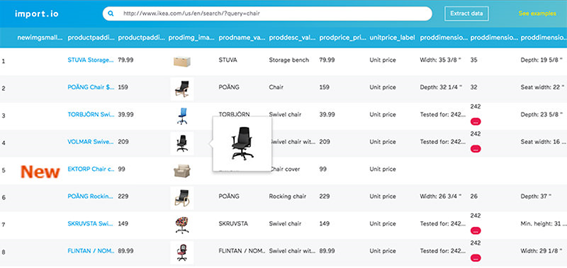
\includegraphics[width=7cm, height=7cm]{imagenes/2.png}


\subsection{Webhose.io}
Webhose.io proporciona acceso directo a datos estructurados y en tiempo real desde 
el rastreo de miles de fuentes en línea. Permite extraer datos web en más de 240 idiomas
 y guardar los datos de salida en varios formatos, incluidos XML, JSON y RSS .
Webhose.io es una aplicación web basada en navegador que utiliza una tecnología
 exclusiva de rastreo de datos para rastrear enormes cantidades de datos de múltiples canales en una única API. Ofrece un plan gratuito para realizar 1000 solicitudes /
 mes y un plan premium de \$ 50 / mes para 5000 solicitudes / mes.
 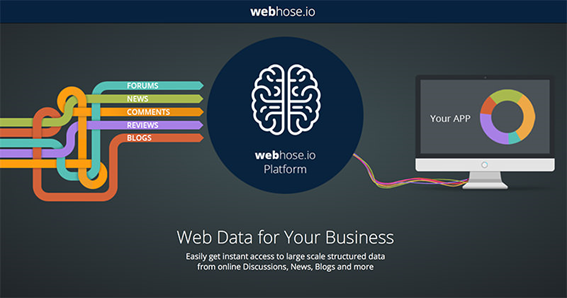
\includegraphics[width=7cm, height=7cm]{imagenes/3.png}

\subsection{Dexi.io (anteriormente conocido como CloudScrape)}
CloudScrape admite la recopilación de datos de cualquier sitio web y no requiere 
descarga como Webhose. 
Proporciona un editor basado en navegador para configurar rastreadores 
y extraer datos en tiempo real. Puede guardar los datos recopilados en plataformas en la nube como Google Drive y Box.net o exportarlos como CSV o JSON.
CloudScrape también admite el acceso anónimo a datos al ofrecer un 
conjunto de servidores proxy para ocultar su identidad. CloudScrape 
almacena sus datos en sus servidores durante 2 semanas antes de archivarlos.
 La herramienta ofrece 20 horas de raspado gratis y tendrá un costo de \$ 29 por mes.
 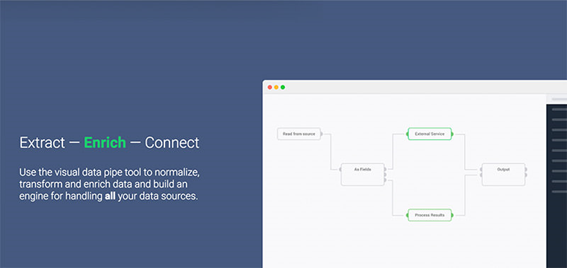
\includegraphics[width=7cm, height=7cm]{imagenes/4.png}

\subsection{Scrapinghub}
Scrapinghub es una herramienta de extracción de datos basada en la nube 
que ayuda a miles de desarrolladores a obtener datos valiosos. Scrapinghub 
usa Crawlera, un rotador de proxy inteligente que admite omitir las contramedidas 
de los bots para rastrear fácilmente 
sitios enormes o protegidos contra bots.
Scrapinghub convierte toda la página web en contenido organizado .
 Su equipo de expertos está disponible para ayudarlo en caso de que 
 su creador de rastreo no pueda satisfacer sus necesidades. Su plan
  básico gratuito le da acceso a 1 rastreo simultáneo y su plan premium por 
  \$ 25 por mes brinda acceso a hasta 4 rastreos paralelos.
  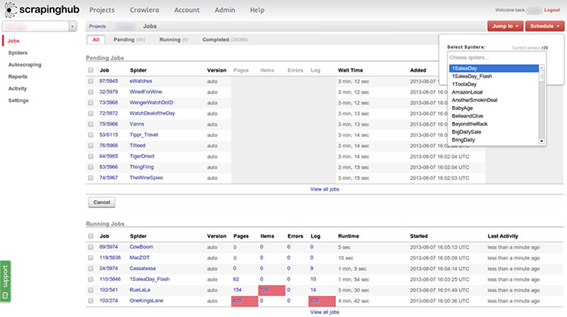
\includegraphics[width=7cm, height=7cm]{imagenes/5.png}

\subsection{ParseHub}
ParseHub está diseñado para rastrear sitios web únicos y múltiples con soporte para 
JavaScript, AJAX, sesiones, cookies y redirecciones. La aplicación utiliza la tecnología
 de aprendizaje automático para reconocer 
los documentos más complicados de la web y genera 
el archivo de salida en función del formato de datos requerido.
ParseHub, además de la aplicación web, también está disponible
 como una aplicación de escritorio gratuita para Windows, 
 Mac OS X y Linux que ofrece un plan básico gratuito que cubre 5 proyectos de rastreo. 
 Este servicio ofrece un plan premium por 
 \$ 89 por mes con soporte para 20 proyectos y 10,000 páginas web por rastreo.
 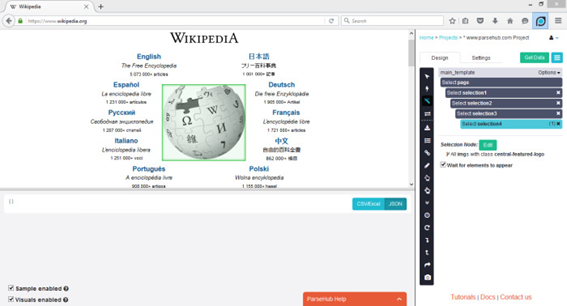
\includegraphics[width=7cm, height=7cm]{imagenes/6.png}

\subsection{VisualScraper}
VisualScraper es otro software de extracción de datos web,
 que se puede utilizar para recopilar información de la web.
  El software lo ayuda a extraer datos de varias páginas web y 
  obtiene los resultados en tiempo real. Además, puede exportar
   en varios formatos como CSV, XML, JSON y SQL .
Puede recopilar y administrar fácilmente los datos web con su 
sencilla interfaz de apuntar y hacer clic . VisualScraper se ofrece
 en forma gratuita, así como en planes premium a partir de \$
  49 por mes con acceso a más de 100K páginas. Su aplicación gratuita,
   similar a la de Parsehub, está disponible para Windows con paquetes
    adicionales de C ++.
    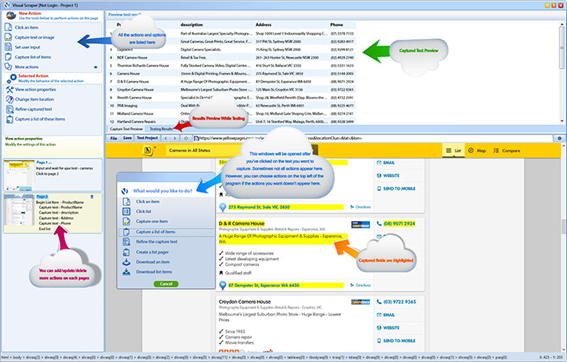
\includegraphics[width=7cm, height=7cm]{imagenes/7.png}

\subsection{Spinn3r}

Spinn3r le permite obtener datos completos de blogs, sitios de noticias y
 redes sociales y feeds RSS y ATOM. Spinn3r se distribuye con una API de
  Firehouse que administra el 95\% del trabajo de indexación. 
  Ofrece una protección avanzada contra el spam, que elimina el 
  spam y los usos inapropiados del lenguaje, lo que mejora la 
  seguridad de los datos.
Spinn3r indexa contenido similar a Google y guarda los datos extraídos
 en archivos JSON. El raspador web escanea constantemente la web y encuentra
  actualizaciones de múltiples fuentes para obtener publicaciones en tiempo real.
   Su consola de administración le permite controlar los rastreos y la búsqueda 
   de texto completo permite realizar consultas complejas en datos sin procesar .
   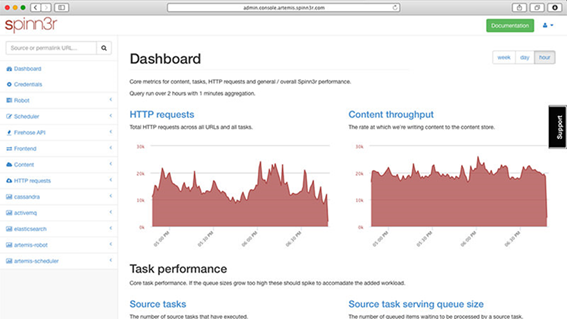
\includegraphics[width=7cm, height=7cm]{imagenes/8.png}


\subsection{80legs}
80legs es una herramienta de rastreo web potente y flexible que se
 puede configurar según sus necesidades. Es compatible con la obtención
  de grandes cantidades de datos, junto con la opción de descargar los
   datos extraídos al instante. El raspador web pretende rastrear más de
    600,000 dominios y es utilizado por grandes jugadores como MailChimp y PayPal.
Su ‘ Datafiniti ‘ le permite buscar rápidamente todos los datos . 80legs
 proporciona un rastreo web de alto rendimiento que funciona rápidamente 
 y recupera los datos requeridos en segundos. Ofrece un plan gratuito para
  10K URL por rastreo y puede actualizarse a un plan de introducción por
   \$ 29 por mes por 100K URL por rastreo.
   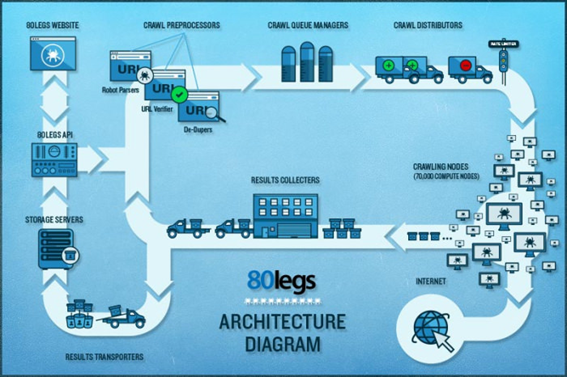
\includegraphics[width=7cm, height=7cm]{imagenes/9.png}


\subsection{Raspador}
Scraper es una extensión de Chrome con funciones limitadas de extracción de datos,
 pero es útil para realizar investigaciones en línea y exportar datos a Google 
 Spreadsheets . Esta herramienta está dirigida a principiantes, así como a expertos
  que pueden copiar fácilmente los datos en el portapapeles o almacenarlos en las 
  hojas de cálculo utilizando OAuth.
Scraper es una herramienta gratuita, que funciona directamente en su navegador y
 genera automáticamente XPaths más pequeños para definir las URL para rastrear. 
 No le ofrece la facilidad de rastreo automático o de bots como Import, Webhose 
 y otros, pero también es un beneficio para los principiantes, ya que no necesita 
 abordar la configuración desordenada .
 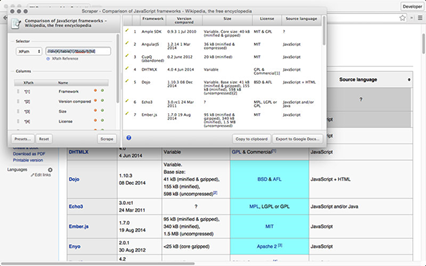
\includegraphics[width=7cm, height=7cm]{imagenes/10.png}



\section{Conclusiones}
En conclusión podríamos decir que la mayoría de los 
conocimientos de una empresa se almacenan de forma no 
estructurada. Las empresas deben posicionarse de cara al 
futuro de forma que hagan accesible el conocimiento a los empleados y 
utilicen los correspondientes métodos escalables. Muchas tecnologías
 prometedoras se están desarrollando de forma rápida y prometedora, 
 especialmente por parte de los startups, y las historias de éxito abundan.
  Quienes consigan abrirse camino en una fase temprana y confiar y comprender
   las nuevas tecnologías no sólo 
podrán mantener su ventaja competitiva, sino incluso ampliarla.
\section{Recomendaciones}
Encontrar la información escondida dentro de los datos no 
estructurados no es una tarea fácil. Requiere análisis avanzado 
y un alto nivel de experiencia técnica para realmente marcar la diferencia. Este puede ser un cambio costoso para muchas empresas.
Sin embargo, quienes pueden aprovechar datos no estructurados
 tienen una ventaja competitiva. Si bien los datos estructurados 
 nos brindan una visión general de los clientes, los datos no
  estructurados pueden brindarnos una comprensión mucho más profunda del comportamiento y la intención del cliente.
Por ejemplo, las técnicas de minería de datos aplicadas a datos 
no estructurados pueden ayudar a las empresas a aprender hábitos 
de compra y tiempos, patrones en las compras, sentimiento hacia un 
producto específico y mucho más.
Los datos no estructurados también son clave para el software de 
análisis predictivo. Por ejemplo, los datos de los sensores conectados 
a la maquinaria industrial pueden alertar a los fabricantes de una actividad 
extraña antes de tiempo. Con esta información, se puede realizar una reparación 
antes de que la máquina sufra una avería costosa.

%----------------------------------------------------------------------------------------
%	REFERENCE LIST
%----------------------------------------------------------------------------------------

\begin{thebibliography}{XXX0000}
	\bibitem - OpenWebinars(Octubre 28, 2019) Qué es MongoDB y características. Recuperado octubre 11, 2021. https://openwebinars.net/blog/que-es-mongodb/ 
	\bibitem - EcuRed(2011) MongoDB. Recuperado Octubre 11, 2021. https://www.ecured.cu/MongoDB 
    \bibitem - MongoDB(2018) La base de datos líder del mercado para aplicaciones modernas.  Recuperado Octubre 11, 2021. https://www.mongodb.com/es 
    \bibitem - Datademia(Noviembre 25, 2020) ¿Qué es MongoDB?  Recuperado Octubre 11, 2021. https://datademia.es/blog/que-es-mongodb 
    \bibitem - ACENS (2014) Bases de datos NoSQL. Qué son y tipos que nos podemos encontrar. Recuperado Octubre 11, 2021. https://www.acens.com/wp-content/images/2014/02/bbdd-nosql-wp-acens.pdf 
    \bibitem - Muradas, Y. (2020) MongoDB vs Redis. Recuperado Octubre 11, 2021. https://openwebinars.net/blog/mongodb-vs-redis/ 
    \bibitem - Garcia,D. (2017) Bases de datos NoSQL. Introducción. Recuperado Octubre 11, 2021. https://ocw.unican.es/pluginfile.php/2396/course/section/2473/Tema\%201.\%20NoSQL\%20introduccio\%CC\%81n.pdf 
    \bibitem - ICHI.PRO(Setiembre 2020) Redis VS MongoDB.   Recuperado Octubre 11, 2021. https://ichi.pro/es/redis-vs-mongodb-196361673285070 
    \bibitem - OpenWebinars(Setiembre 14, 2020) MongoDB vs Redis. Recuperado Octubre 11, 2021. https://openwebinars.net/blog/mongodb-vs-redis/ 
    \bibitem - Moreno,F , Quintero,J , Rueda,R (2016) Una comparación de rendimiento entre Oracle y MongoDB. Recuperado Octubre 11, 2021. http://www.scielo.org.co/scielo.php

	\end{thebibliography}

%----------------------------------------------------------------------------------------

\end{document}